\subsection{Architecture generation}
\begin{frame}
	\frametitle{Architecture generation}
	toto is happier.
\end{frame}

\begin{frame}
	\frametitle{Example}
	\begin{figure}
		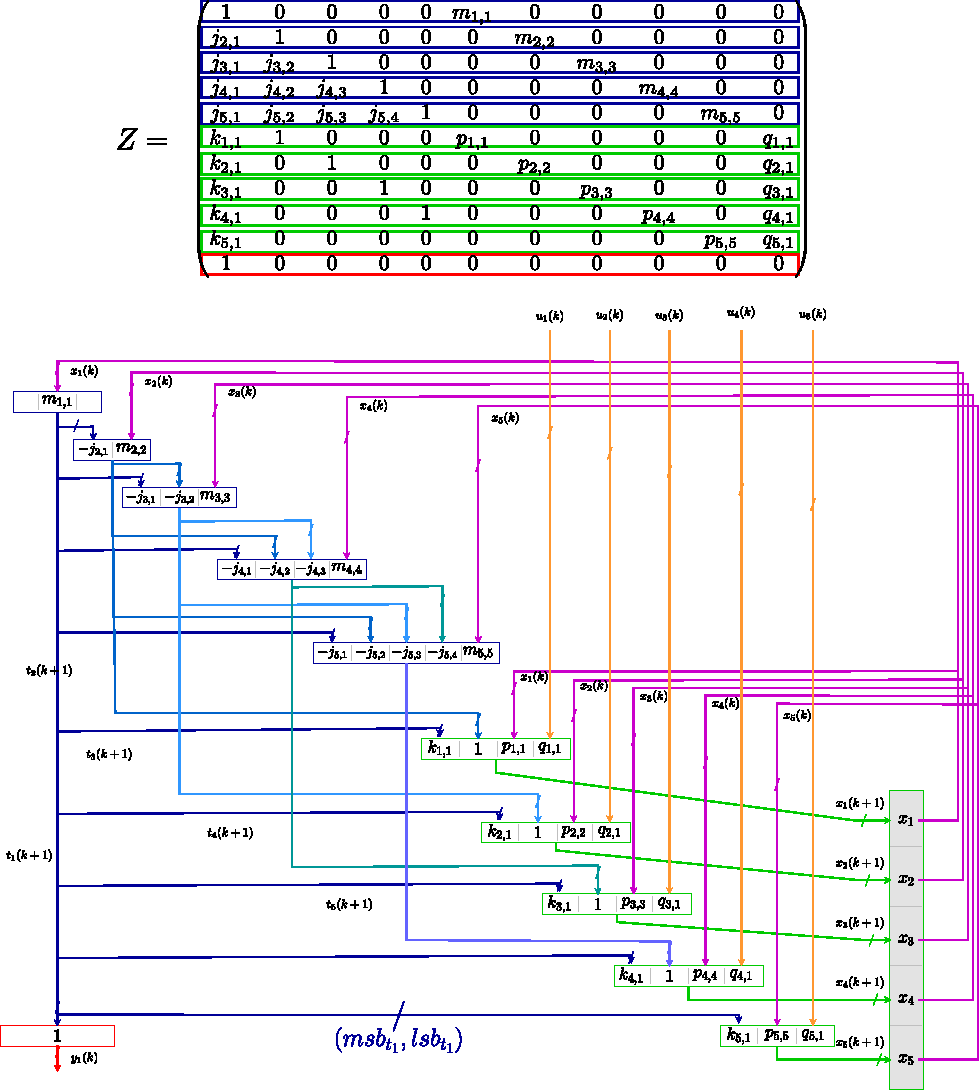
\includegraphics[scale=0.4]{pictures/exampleFull.pdf}
	\end{figure}
\end{frame}

\begin{frame}
	\frametitle{Example}
	\begin{figure}
	  \begin{tikzpicture}

		%\normalsize 
		\footnotesize
		\node[draw, blue!100, thick, rectangle, minimum width =6.5cm, minimum height=0.25cm] (sel1)  at (5,1.55) {} ;
		\node[draw, blue1!100, thick, rectangle, minimum width =6.5cm, minimum height=0.25cm] (sel2)  at (5,1.25) {} ;
		\node[draw, blue2!100, thick, rectangle, minimum width =6.5cm, minimum height=0.25cm] (sel3)  at (5,0.95) {} ;
		\node[draw, blue3!100, thick, rectangle, minimum width =6.5cm, minimum height=0.25cm] (sel4)  at (5,0.64) {} ;
		\node[draw, blue4!100, thick, rectangle, minimum width =6.5cm, minimum height=0.25cm] (sel5)  at (5,0.33) {} ;
		\node[draw, green!100, thick, rectangle, minimum width =6.5cm, minimum height=0.25cm] (sel6)  at (5,0) {} ;
		\node[draw, green!100, thick, rectangle, minimum width =6.5cm, minimum height=0.25cm] (sel7)  at (5,-0.30) {} ;
		\node[draw, green!100, thick, rectangle, minimum width =6.5cm, minimum height=0.25cm] (sel8)  at (5,-0.62) {} ;
		\node[draw, green!100, thick, rectangle, minimum width =6.5cm, minimum height=0.25cm] (sel9)  at (5,-0.93) {} ;
		\node[draw, green!100, thick, rectangle, minimum width =6.5cm, minimum height=0.25cm] (sel10) at (5,-1.25) {} ;
		\node[draw, red!100, thick, rectangle, minimum width =6.5cm, minimum height=0.25cm] (sel11) at (5,-1.55) {} ;

		\node at (0, 0) { \huge $Z = $};
		\normalsize
	  \node at (5, 0) {
		\resizebox{200pt}{!}{
			$\begin{pmatrix}
				1       & 0       & 0       & 0       & 0       & \textcolor{purple}{m_{1,1}} & 0       & 0       & 0       & 0       & 0       \\
				j_{2,1} & 1       & 0       & 0       & 0       & 0       & \textcolor{purple}{m_{2,2}} & 0       & 0       & 0       & 0       \\
				j_{3,1} & j_{3,2} & 1       & 0       & 0       & 0       & 0       & \textcolor{purple}{m_{3,3}} & 0       & 0       & 0       \\
				j_{4,1} & j_{4,2} & j_{4,3} & 1       & 0       & 0       & 0       & 0       & \textcolor{purple}{m_{4,4}} & 0       & 0       \\
				j_{5,1} & j_{5,2} & j_{5,3} & j_{5,4} & 1       & 0       & 0       & 0       & 0       & \textcolor{purple}{m_{5,5}} & 0       \\
				k_{1,1} & 1       & 0       & 0       & 0       & \textcolor{purple}{p_{1,1}} & 0       & 0       & 0       & 0       & \textcolor{orange}{q_{1,1}} \\

				k_{2,1} & 0       & 1       & 0       & 0       & 0       & \textcolor{purple}{p_{2,2}} & 0       & 0       & 0       & \textcolor{orange}{q_{2,1}} \\
				k_{3,1} & 0       & 0       & 1       & 0       & 0       & 0       & \textcolor{purple}{p_{3,3}} & 0       & 0       & \textcolor{orange}{q_{3,1}} \\
				k_{4,1} & 0       & 0       & 0       & 1       & 0       & 0       & 0       & \textcolor{purple}{p_{4,4}} & 0       & \textcolor{orange}{q_{4,1}} \\
				k_{5,1} & 0       & 0       & 0       & 0       & 0       & 0       & 0       & 0       & \textcolor{purple}{p_{5,5}} & \textcolor{orange}{q_{5,1}} \\

				1	    & 0       & 0       & 0       & 0       & 0       & 0       & 0       & 0       & 0       & 0       \\
			\end{pmatrix}$
	  }
	  };

		\end{tikzpicture}
	\end{figure}
\end{frame}


\begin{frame}
	\frametitle{Example}
	\begin{figure}
		%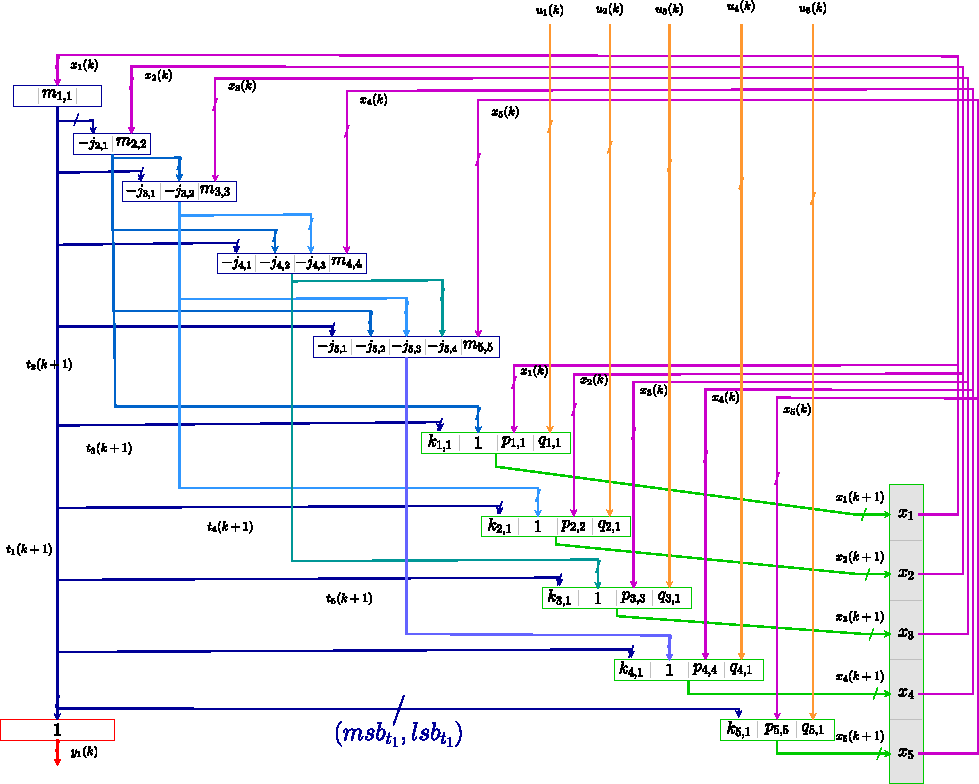
\includegraphics[scale=0.8]{pictures/exampleScheme.pdf}
		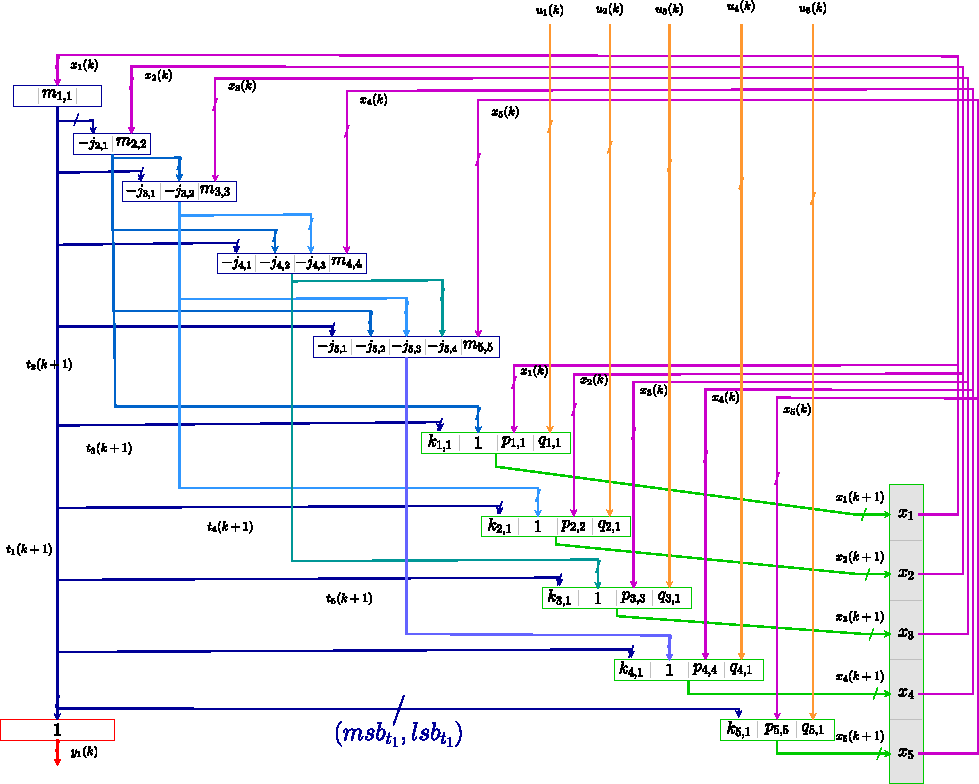
\includegraphics[scale=0.7, trim=0cm 5cm 2cm 0cm,clip]{pictures/exampleScheme.pdf}
	\end{figure}
\end{frame}

\begin{frame}
	\frametitle{Example}
	\begin{figure}
		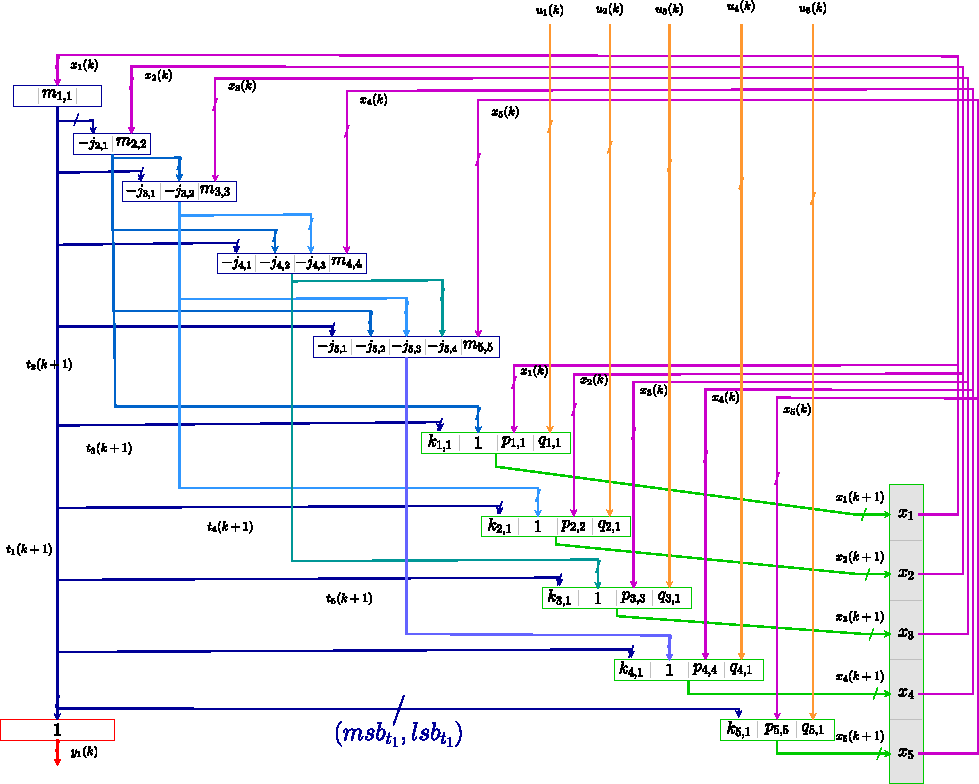
\includegraphics[scale=0.8, trim=5cm 0cm 0cm 5cm,clip]{pictures/exampleScheme.pdf}
	\end{figure}
\end{frame}
